\section{Data construction}
\label{sec:data}
The section describes the construction of the dataset used for this work. It includes a description of the necessity of constructing the data from scratch, the source of the audio used, and the construction of the trials. 

\subsection{Why the data is constructed}
\label{sec:construct}
There are three main considerations for the dataset that need to be met: \textit{(i)} training requires a clean target signal as a reference for what the extractor should output, \textit{(ii)} the data must possess exact transcriptions of the target signal to allow for transcription-based evaluation, and \textit{(iii)} the data must possess both best case and worst case scenarios in order to interpret the performance of the extractor relative to these scenarios. These considerations limit the available choices of publically available datasets.

Constructing the data is also the established practice. The 2026 REAL-TSE challenge \cite{wang2026realtse} supplied no training set at all, and required that participants document whichever open-source data they used. The organisers after reviewing the submissions, describe the data recipe that the entrants converged on:

\begin{quote}
``Most teams synthesized mixtures from publicly available speech corpora such as LibriSpeech\ldots; added noise from WHAM!\ldots; and introduced reverberation with measured/simulated RIRs, while varying the number of speakers, SNR/SIR, RT60, chunk length, and enrollment quality. Many teams also injected target-absent or noise-only segments, forcing systems not only to extract the target when present but also to suppress non-target speech and avoid false extraction.''
\hfill\cite{wang2026realtse}
\end{quote}

The dataset constructed here follows that recipe, and the sections below describe each of its components in turn. The organisers further observed that several of the strongest entries were built on backbones near-identical to the official baseline architecture, the BSRNN, yet scored substantially better. They attribute the success to data simulation, real-data adaptation, pseudo-label filtering, loss design and post-processing rather than to architecture alone.    

\subsection{Source of audio}
\label{sec:audio}
The audio data was collected from a variety of sources to produce a diverse dataset. Speech was chosen for target and interferer from the LibriSpeech \cite{panayotov2015librispeech} dataset, which is a corpus of read English speech derived from audiobooks. The background noise was chosen from WHAM! \cite{wichern2019wham} which is a dataset of real-world noise recordings considering environments such as offices, streets, and cafés. 


\subsection{Trial construction}
\label{sec:trial_construction}
The trials are structured in a way to replicate the conditions of a real-world target speaker extraction scenario. Due to the difficulty of the TSE task, it was decided that the data should reflect a variety of conditions, but primarily focus on the base case task of a target speaker close to a recording device with an interfering speaker in a similar proximity and faint background noise. The difficulty came in constructing the dataset to be realistic enough to simulate a real-world scenario, but also not so difficult that a simple extractor of limited capacity would be unable to learn the task. A visual representation of the trial construction can be found in Figure \ref{fig:trial_construction}.
\begin{figure}[h]
    \centering
    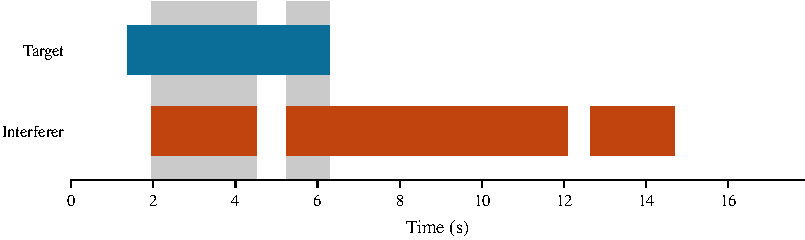
\includegraphics[width=0.7\textwidth]{figures/trial_timeline_low_overlap.pdf}
    \caption{Visual representation of the trial construction. The target and interferer are drawn from LibriSpeech, and the noise bed is drawn from WHAM!. The shaded areas show the overlapping regions of speech.}
    \label{fig:trial_construction}
\end{figure} 

A single trial consists of the following components: \textit{(i)} target speech, \textit{(ii)} interferer speech, \textit{(iii)} noise bed, \textit{(iv)} the mixture of the first three components, and \textit{(v)} an enrollment clip of the target speaker. The trial belongs to one of four conditions: both speakers present, only the target speaker present, only the interferer speaker present, and neither speaker present. The mixture is constructed to be 15-20 seconds long. The trials are drawn from two separate regimes: a base case and a difficult case. The base case is constructed to be a simple but realistic scenario, and difficult cases are edge cases that are constructed to be more challenging for the extractor. There are two both male and female speakers in the dataset. To simulate room acoustics, including reverberation, room dimensions, source and microphone positions, the \texttt{pyroomacoustics} \cite{scheibler2018pyroomacoustics} package is used to simulate the room impulse response. The trials are constructed to be as realistic as possible, but also to be reproducible and controllable. A sample of the room construction can be found in the Appendix \ref{sec:room_construction}. 

\paragraph{Enrollment.} [TODO validatae the enrollment clip length and whether it is a single clip or multiple clips]
The enrollment clip is a short audio segment of the target speaker. The clip is used to provide the extractor with a reference of what the target speaker sounds like. The clips are taken from the same source as the target speech, which is LibriSpeech. To avoid bias in the extractor, the enrollment clip is first attempted to be drawn from a different book reading. If this is unsuccessful, then the clip is drawn from a different chapter of the same book. Finally, if this is also unsuccessful, then the clip is drawn from a different utterance of the same chapter. The reason for this is to avoid the extractor memorising the target speech by learning to recognise the content rather than the \emph{manner} that the target speaker speaks. The distribution of enrollment clips across the dataset is shown in Figure \ref{fig:enrollment_distribution}. Again to avoid bias, the enrollment clips are simulated to come from different recording devices. This is done by applying equalisation (EQ) augmentation to the enrollment clips by applying a random EQ filter to the clip with a probability of \num{0.5}. This technique was suggested by the CARTSE \cite{li2026cartse} submission for the 2026 REAL-TSE challenge \cite{wang2026realtse}.
\begin{figure}[h]
    \centering
    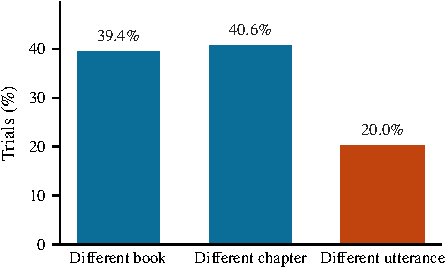
\includegraphics[width=0.7\textwidth]{figures/enrollment_provenance.pdf}
    \caption{Distribution of the source of the enrollment clips across the dataset.}
    \label{fig:enrollment_distribution}
\end{figure}


\paragraph{Parameter distribution choice.}
The Signal-to-Interference Ratio (SIR) is chosen uniformly from the range of -10 to 10 dB, and the Signal-to-Noise Ratio (SNR) is chosen uniformly from the range of 0 to 20 dB. These two ratios simulate the relative loudness of the target speaker to the interferer and background noise, respectively. A negative number for the SIR indicates that the interferer is louder than the target speaker, and the lower the SNR, the louder the background noise is relative to the target speaker. The SIR was chosen to be symmetric around \SI{0}{\decibel} after experimentation found that if the target was always (or majority of the time) louder than the interferer, then the extractor would just learn to follow the speech that was loudest and hence ignore the conditioning of the enrollment audio. This defeats the purpose of the task hence the stated requirement.

The reverberation of each room is set by a reverberation time, $T_{60}$, which is defined to be the time it takes for sound to decay by \SI{60}{\decibel}. The larger the value the more reverberant the room is. $T_{60}$ is drawn from a uniform distribution between \SIrange{0.25}{0.6}{\second}, which are values that span a carpeted office to a larger room with hard surfaces. To enforce realism, the absorption rate of the walls is also considered. The absorption rate is considered using the Sabine relation \cite{sabine1922}. The relation connects the physical properties of a room to its volume, its surface area and the absorption of its surfaces, so once the dimensions and the $T_{60}$ have been drawn the absorption is fixed by them and is solved for rather than sampled. A draw is rejected and replaced if the requested $T_{60}$ is not achievable in a room of the drawn size, which is also the reason for the lower bound of \SI{0.25}{\second}.

The remaining parameters and their distributions can be found in the Appendix \ref{app:params} 

\paragraph{Target-absent trials.} The extractor needs example trials to learn to rely on the conditioning of the enrollment audio to identify target speech. The target-absent trials support this idea by having the model learn to stay silent when the enrollment speaker is not present. The split is as follows for these trials: 49.5\% both speakers present, 25.5\% target only, 19.6\% interferer only and 5.4\% noise only.

\paragraph{Splits.} The dataset is split into a training and validation sets. Each of these sets have their own distinct set of speakers such that there is no overlap of speakers between the sets. The training set consists of \num{9955} trials, consisting of \num{1172} unique speakers. The validation set consists of \num{200} trials drawn from \num{40} speakers. The idea behind this is to ensure that the model does not memorise speakers, but rather to learn to extract the target speaker based on the enrollment clip. Finally, in a final evaluation holdout set, there are no target-absent trials. The training split was progressively built up in stages from \num{1989} to \num{4976} and then finally to \num{9955} trials. This was done to measure the effect of the quantity of data on the performance of the extractor. The final evaluation holdout set consists of \num{103} trials.

\paragraph{Limitations.} The dataset is constructed to be as realistic as possible, but it is still a simulated dataset. The dataset is restricted to two speakers, which can confound the extractor to expect the target to be present if two speakers are present. Secondly, the combined audio forms \emph{read} speech and not \emph{conversational} speech. This means that the resulting audio does not have natural turn-taking, or conversational dynamics. These dynamics are simulated through the overlap of the target and interferer, but it is not a perfect simulation. Next, the dataset is restricted to English speech, and shoebox rooms only. Finally, the noise beds use are from WHAM! \cite{wichern2019wham} and range in length from 5 to 20 seconds long. This means that the noise beds are not long enough occassionally to cover the entire trial. To solve this, the noise bed is looped to cover the entire trial. 

